\documentclass{article}
\usepackage{graphicx} % Required for inserting images
\usepackage[utf8]{inputenc}
\usepackage{setspace}
\usepackage[margin=1.5cm]{geometry}
\usepackage{amsmath}
\usepackage{amsthm}
\usepackage{amsfonts}
\usepackage{indentfirst}
\usepackage{tikz}

\title{Regions in the Complex Plane}
\author{Matthew Seguin}
\date{}

\begin{document}

\maketitle

\section*{6.9}
\begin{center}
    \doublespacing
    Assume $|z| = 2$. Then consider $w = z^4 - 4z^2 + 3$. Recall that for $z_1, z_2\in\mathbb{C}$ we know $||z_1| - |z_2||\leq |z_1 + z_2|$.
    \\By factoring we get $w = z^4 - 4z^2 + 3 = (z^2 - 1)(z^2 - 3)$.
    \\Therefore $|w| = |(z^2 - 1)(z^2 - 3)| = |z^2 - 1||z^2 - 3|\geq (||z^2| - |-1||)|z^2 - 3| = (||z|^2 - 1|)|z^2 - 3| = (|4 - 1|)|z^2 - 3| = 3|z^2 - 3|\geq 3||z^2| - |-3|| = 3||z|^2 - 3| = 3|4 - 3| = 3$.
    \\So we have that $|w| = |z^4 - 4z^2 + 3|\geq 3$ and hence $\frac{1}{|w|} =\frac{1}{|z^4 - 4z^2 + 3|}\leq\frac{1}{3}$.
    \\Therefore since $|w^{-1}| = |\frac{1}{w}| =\frac{1}{|w|}$ we get:
    \\$|\frac{1}{z^4 - 4z^2 + 3}| =\frac{1}{|z^4 - 4z^2 + 3|}\leq\frac{1}{3}$ \qedsymbol
\end{center}


\section*{6.14}
\begin{center}
    \doublespacing
    Let $S =\{z = x + iy: x^2 - y^2 = 1\}$. Recall that for $z_1, z_2, z_3, z_4\in\mathbb{C}$ we know $(\frac{z_1}{z_2})(\frac{z_3}{z_4}) =\frac{z_1 z_3}{z_2 z_4}$.
    \\Recall that for any $z\in\mathbb{C}$ we have $Re\:z =\frac{z +\overline{z}}{2}$ and $Im\:z =\frac{z -\overline{z}}{2i}$.
    \\Therefore if $z\in S$ we have $x^2 - y^2 = (Re\:z)^2 - (Im\:z)^2 = 1$.
    \\So for $z\in S$ we have $(Re\:z)^2 - (Im\:z)^2 = (\frac{z +\overline{z}}{2})^2 - (\frac{z -\overline{z}}{2i})^2 = (\frac{z +\overline{z}}{2})(\frac{z +\overline{z}}{2}) - (\frac{z -\overline{z}}{2i})(\frac{z -\overline{z}}{2i}) =\frac{z^2 + 2z\overline{z} +\overline{z}^2}{4} -\frac{z^2 - 2z\overline{z} +\overline{z}^2}{4i^2} =\frac{z^2 + 2z\overline{z} +\overline{z}^2}{4} +\frac{z^2 - 2z\overline{z} +\overline{z}^2}{4} =\frac{2(z^2 +\overline{z}^2)}{4} =\frac{z^2 +\overline{z}^2}{2} = 1$.
    \\Therefore $z^2 +\overline{z}^2 = 2$ and without loss of generality we can say the same is true in reverse so $z\in S$ if and only if $z^2 +\overline{z}^2 = 2$. Hence $S =\{z\in\mathbb{C}: z^2 +\overline{z}^2 = 2\}$.
    \\Since $S$ is all the points lying on a hyperbola we have that $z^2 +\overline{z}^2 = 2$ defines the same hyperbola \qedsymbol
\end{center}


\newpage
\section*{9.4}
\begin{center}
    \doublespacing
    Recall that for a complex number $z = r e^{i\theta}$ the expression $|z - 1| = |r e^{i\theta} - 1|$ represents the distance of $z$ from 1.
    \\We want to find a point $z = e^{i\theta}$ such that $|e^{i\theta} - 1| = 2$ where $\theta\in [0, 2\pi)$.
    \\Since $z = e^{i\theta}$ we get that $r = |z| = |e^{i\theta}| = |cos(\theta) + i\:sin(\theta)| =\sqrt{cos^2 (\theta) + sin^2 (\theta)} = 1$.
    \\So we are looking for a complex number lying on the unit circle centered at 0 whose distance from 1 is 2.
    \\We know that 1 is a point on the unit circle centered at 0 and that it makes an angle 0 with the real axis since $1\in\mathbb{R}$.
    \\Therefore the only point on the unit circle centered at 0 that can be a distance of 2 away from 1 is the point on the opposite side of the unit circle centered at 0. This is because the diameter of the unit circle centered at 0 is 2.
    \break
    \\So the angle between these two points will be $\pi$ because this will take us half way around the circle.
    \\Since 1 makes an angle of 0 with the real axis we get that $arg\:z =\{\pi + 2n\pi: n\in\mathbb{Z}\}$.
    \\The only one of these angles in the interval $[0, 2\pi)$ is when $n = 0$ and hence $\theta =\pi$ \qedsymbol
    \break
    \\You can see this algebraically too:
    \\We want $|z - 1| = 2$ where $z = e^{i\theta}$ and hence $|z| = 1$.
    \\So $|z - 1|^2 = 4$ and $(z-1)(\overline{z-1}) = (z-1)(\overline{z} - 1) = z\overline{z} - z -\overline{z} + 1 = 4$.
    \\Therefore $|z|^2 - 2 Re\:z = 1 - 2 Re\:z = 3$. Giving $Re\:z = -1$.
    \\Then if $Re\:z = -1$ we must have $(Re\:z)^2 + (Im\:z)^2 = 1 + (Im\:z)^2 = 1$. Hence $Im\:z = 0$ and $z = -1$.
    \\This means $z = -1 = cos(\theta) + i\:sin(\theta)$ gives $cos(\theta) = -1$ and $sin(\theta) = 0$ for $\theta\in [0, 2\pi)$.
    \\So $\theta =\pi$ as desired.
\end{center}


\section*{9.8}
\begin{center}
    \doublespacing
    As given in the problem $(e^{i\frac{\theta _1 +\theta _2}{2}})(e^{i\frac{\theta _1 -\theta _2}{2}}) = e^{i\theta _1}$ and $(e^{i\frac{\theta _1 +\theta _2}{2}})(\overline{e^{i\frac{\theta _1 -\theta _2}{2}}}) = e^{i\theta _2}$.
    \\Let $z_1, z_2\in\mathbb{C}$. Recall that for $w, w_1, w_2\in\mathbb{C}$ we know $|w_1 w_2| = |w_1||w_2|$ and $|w| = |\overline{w}|$.
    \begin{itemize}
        \item Assume $r_1 = |z_1| = |z_2| = r_2 = r$:
    \end{itemize}
    Represent $z_1$ and $z_2$ as $r e^{i\theta _1}$ and $r e^{i\theta _2}$ respectively.
    \\Then $z_1 = r e^{i\theta _1} = r (e^{i\frac{\theta _1 +\theta _2}{2}})(e^{i\frac{\theta _1 -\theta _2}{2}})$ and $z_2 = r e^{i\theta _2} = r (e^{i\frac{\theta _1 +\theta _2}{2}})(\overline{e^{i\frac{\theta _1 -\theta _2}{2}}})$.
    \\Let $c_1 = r e^{i\frac{\theta _1 +\theta _2}{2}}$ and $c_2 = e^{i\frac{\theta _1 -\theta _2}{2}}$. Then we have $z_1 = c_1 c_2$ and $z_2 = c_1\overline{c_2}$.
    \\So there exists $c_1, c_2\in\mathbb{C}$ such that $z_1 = c_1 c_2$ and $z_2 = c_1\overline{c_2}$.
    \begin{itemize}
        \item Assume there exists $c_1, c_2\in\mathbb{C}$ such that $z_1 = c_1 c_2$ and $z_2 = c_1\overline{c_2}$:
    \end{itemize}
    Then $|z_1| = |c_1 c_2| = |c_1||c_2| = |c_1||\overline{c_2}| = |c_1\overline{c_2}| = |z_2|$.
    \break
    \\This was for arbitrary $z_1, z_2\in\mathbb{C}$ and is therefore true for all $z_1, z_2\in\mathbb{C}$.
    \\So for $z_1, z_2\in\mathbb{c}$ we have that $|z_1| = |z_2|$ if and only if $z_1 = c_1 c_2$ and $z_2 = c_1\overline{c_2}$ for some $c_1, c_2\in\mathbb{C}$ \qedsymbol
\end{center}


\newpage
\section*{9.10}

{\Large\textbf{a.}} Recall that de Moivre's formula says $(cos(\theta) + i\:sin(\theta))^n = cos(n\theta) + i\:sin(n\theta)$.
\begin{center}
    \doublespacing
    Recall the binomial theorem where for $z_1, z_2\in\mathbb{C}$ we know \[(z_1 + z_2)^n =\sum _{k=0}^n\binom{n}{k} z_1^k z_2^{n-k}\]
    \\Consider $(cos(\theta) + i\:sin(\theta))^3$. We can apply the binomial theorem with $z_1 = cos(\theta)$ and $z_2 = i\:sin(\theta)$.
    \\Then we get $(cos(\theta) + i\:sin(\theta))^3 =\binom{3}{0} (i\:sin(\theta))^3 +\binom{3}{1} (cos(\theta))(i\:sin(\theta))^2 +\binom{3}{2} (cos(\theta))^2(i\:sin(\theta)) +\binom{3}{3} (cos(\theta))^3 = (cos^3 (\theta) - 3 cos(\theta)sin^2(\theta)) + i(3\:cos^2(\theta)sin(\theta) -sin^3(\theta))$.
    \break
    \\But we also know from de Moivre's formula that $(cos(\theta) + i\:sin(\theta))^3 = cos(3\theta) + i\:sin(3\theta)$.
    \\Therefore $(cos^3 (\theta) - 3 cos(\theta)sin^2(\theta)) + i(3\:cos^2(\theta)sin(\theta) -sin^3(\theta)) = cos(3\theta) + i\:sin(3\theta)$.
    \\Hence $Re\:((cos^3 (\theta) - 3 cos(\theta)sin^2(\theta)) + i(3\:cos^2(\theta)sin(\theta) -sin^3(\theta))) = Re\:(cos(3\theta) + i\:sin(3\theta))$.
    \\So $cos^3 (\theta) - 3 cos(\theta)sin^2 (\theta) = cos(3\theta)$ as desired \qedsymbol
\end{center}


\section*{11.6}
\begin{center}
    \doublespacing
    Recall that the $n$ distinct $n$th roots of $z\in\mathbb{C}$ are given by $c_k = \sqrt[n]{|z|} e^{i(\frac{Arg\:z}{n} +\frac{2k\pi}{n})} = \sqrt[n]{|z|} e^{i\frac{Arg\:z}{n}} e^{i\frac{2k\pi}{n}} = c_0 w_n^k$
    \\where $c_0$ is the principle root, $w_n = e^{i\frac{2\pi}{n}}$, and $k\in\{0, 1, 2, ..., n-1\}$.
    \break
    \\We are looking for the 4 distinct solutions to $z^4 + 4 = 0$ and hence the 4 distinct 4th roots of -4.
    \\We are given $z_0 =\sqrt{2} e^{i\frac{\pi}{4}} = 1 + i$ is the principle 4th root of -4.
    \\Now $w_4 = e^{i\frac{2\pi}{4}} = e^{i\frac{\pi}{2}} = cos(\frac{\pi}{2}) + i\:sin(\frac{\pi}{2}) = i$.
    \\So we have our distinct roots are:
    \\$z_0 = 1 + i$
    \\$z_1 = z_0 w_4 = (1 + i)i = i + i^2 = -1 + i$
    \\$z_2 = z_0 w_4^2 = (1 + i)i^2 = -(1 + i) = -1 - i$
    \\$z_3 = z_0 w_4^3 = (1 + i)i^3 = -i(1 + i) = -i - i^2 = 1 - i$
    \break
    \\First notice that $z_3 =\overline{z_0}$ and $z_2 =\overline{z_1}$.
    \\We can deconstruct $z^4 + 4$ into its roots.
    \\$z^4 + 4 = (z - z_0)(z - z_1)(z - z_2)(z - z_3) = (z - z_0)(z -\overline{z_0})(z - z_1)(z -\overline{z_1}) =$
    \\$(z^2 - z\overline{z_0} - z z_0 + z_0\overline{z_0})(z^2 - z\overline{z_1} - z z_1 + z_1\overline{z_1}) = (z^2 - z(z_0 +\overline{z_0}) + |z_0|^2)(z^2 - z(z_1 -\overline{z_1}) + |z_1|^2) =$
    \\$(z^2 - (2 Re\:z_0) z + |z_0|^2)(z^2 - (2 Re\:z_1) z + |z_1|^2) = (z^2 - 2z + 2)(z^2 + 2z + 2)$ \qedsymbol
\end{center}


\newpage
\section*{11.7}
\begin{center}
    \doublespacing
    Recall that from problem 9 of section 9 for $z\neq 1$ we have $1 + z + z^2 + ... + z^n =\frac{1 - z^{n+1}}{1 - z}$.
    \\Let $n\in\mathbb{N}$ and $c\in\mathbb{C}$ such that $c\neq 1$ and $c^n = 1$. Then $c$ is a so-called $n$th root of unity.
    \\Since $c\neq 1$ we have that $1 + c + c^2 + ... + c^{n-1} =\frac{1 - c^n}{1 - c} =\frac{1 - 1}{1 - c} =\frac{0}{1 - c} = 0$ as desired.
    \\This was for arbitrary $n\in\mathbb{N}$ and for arbitrary $c\neq 1$ where $c^n = 1$, so $1 + c + c^2 + ... + c^{n-1} = 0$
    \\for all $n$th roots of unity $c\neq 1$ \qedsymbol
    \break
    \\Geometrically this makes sense as well:
    \\The $n$ distinct $n$th roots of unity are spread evenly along the unit circle.
    \\Once you fix one root $c\neq 1$ you can find the other $n-1$ roots are $c^2, c^3, ..., c^n$ where $c^n = 1$.
    \\Therefore by adding all of these terms you are adding all of the evenly spaced roots on the unit circle, which will necessarily add to 0 by the nature of vectors.
    \\Actually, for any $z\in\mathbb{C}$ and any $n\in\mathbb{N}$ where $n\geq 2$ the sum of the $n$ distinct $n$th roots of $z$ will add to 0 because they are evenly spaced along the same circle. We simply get that when $z = 1$ it is a special case where all the roots can be represented as $c, c^2, c^3, ..., c^n$ where $c\neq 1$ is one of the $n$th roots of unity.
    \break
    \\Proof that $1 + z + z^2 + ... + z^n =\frac{1 - z^{n+1}}{1 - z}$ for $z\neq 1$ (result from P9 of Sec. 9):
    \\Recall that the familiar distributive laws apply just the same in the complex numbers as in the real numbers.
    \\Let $z\neq 1$ then consider the product $(1 - z)(1 + z + z^2 + ... + z^n)$.
    \\We can write $(1 - z)(1 + z + z^2 + ... + z^n) = (1 + z + z^2 + ... + z^n) - z(1 + z + z^2 + ... + z^n) = (1 + z + z^2 + ... + z^n) - (z + z z + z z^2 + ... + z z^n) = (1 + z + z^2 + ... + z^n) - (z + z^2 + z^3 + ... + z^{n+1}) = 1 + z + z^2 + ... + z^n - z - z^2 - z^3 + ... - z^{n+1} = 1 + (z - z) + (z^2 - z^2) + ... + (z^n - z^n) - z^{n+1} = 1 - z^{n+1}$.
    \\Then since $z\neq 1$ we have $z - 1\neq 0$ and we can divide both sides by $z - 1$.
    \\So $\frac{(1 - z)(1 + z + z^2 + ... + z^n)}{1 - z} = 1 + z + z^2 + ... + z^n =\frac{1 - z^{n+1}}{1 - z}$ as desired.
\end{center}


\section*{11.8}

{\Large\textbf{a.}} Let $z\in\mathbb{C}$ then consider the equation $a z^2 + b z + c = 0$ where $a, b, c\in\mathbb{C}$ and $a\neq 0$.
\begin{center}
    \doublespacing
    Then we get $a z^2 + b z = -c$ and $z^2 +\frac{b}{a} z = -\frac{c}{a}$ (we can divide by $a$ since $a\neq 0$).
    \\Then $z^2 + 2\frac{b}{2a} z = -\frac{c}{a}$ and  $z^2 + 2\frac{b}{2a} z + (\frac{b}{2a})^2= (\frac{b}{2a})^2 -\frac{c}{a}$.
    \\So $(z +\frac{b}{2a})^2 =\frac{b^2}{4a^2} -\frac{c}{a} =\frac{b^2}{4a^2} -\frac{4ac}{4a^2} =\frac{b^2 - 4ac}{4a^2}$.
    \\Therefore $z +\frac{b}{2a} = ((z +\frac{b}{2a})^2)^{\frac{1}{2}} =\pm (\frac{b^2 - 4ac}{4a^2})^{\frac{1}{2}} =\pm\frac{(b^2 - 4ac)^{\frac{1}{2}}}{(4a^2)^{\frac{1}{2}}} =\pm\frac{(b^2 - 4ac)^{\frac{1}{2}}}{2a}$.
    \\Since there are only 2 second roots for any complex number, the principal root and its rotation by $\frac{2\pi}{2} =\pi$ (its negative).
    \\And finally $z = -\frac{b}{2a}\pm\frac{(b^2 - 4ac)^{\frac{1}{2}}}{2a} =\frac{- b\pm(b^2 - 4ac)^{\frac{1}{2}}}{2a}$ as desired \qedsymbol
\end{center}


\newpage
\section*{12.1}

{\Large\textbf{a.}} Let $S =\{z\in\mathbb{C}: |z - 2 + i|\leq 1\} =\{z\in\mathbb{C}: |z - (2 - i)|\leq 1\}$.
\begin{center}
    \doublespacing
    Then $S$ consists of all the points that are at most a distance of 1 away from the point $2 - i$.
    \break
    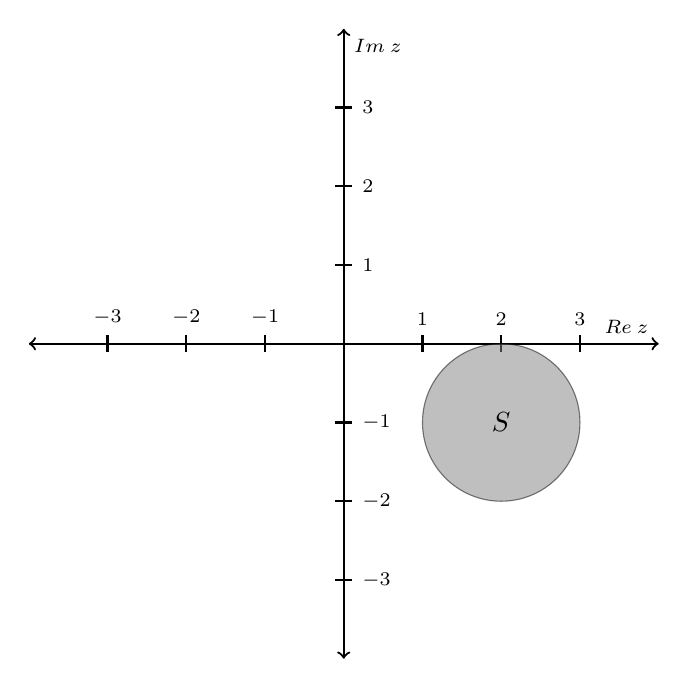
\begin{tikzpicture}
    \begin{scope}[thick,font=\scriptsize]
    \draw [<->] (-4,0) -- (4,0) node [above left]  {$Re\:z$};
    \draw [<->] (0,-4) -- (0,4) node [below right] {$Im\:z$};
    \foreach \n in {-3,...,-1,1,2,...,3}{
        \draw (\n,-3pt) -- (\n,3pt)   node [above] {$\n$};
        \draw (-3pt,\n) -- (3pt,\n)   node [right] {$\n$};
    }
    \end{scope}
    \path [draw=black,fill=gray,semitransparent] (+2,-1) circle (1);
    \node [black] at (+2,-1) {$S$};
    \end{tikzpicture}
    \\Clearly the boundary of $S$ is given by $\{z\in\mathbb{C}: |z - (2 - i)| = 1\}\subseteq S$.
    \\Therefore $S$ contains all its boundary points and hence is not open. So $S$ is not a domain.
\end{center}

{\Large\textbf{e.}} Let $S =\{z\in\mathbb{C}: 0\leq arg\:z\leq\frac{\pi}{4}\}$.
\begin{center}
    \doublespacing
    I am assuming this is referring to $z$'s principle argument otherwise the inequalities don't make sense.
    \\Then $S$ consists of all the points whose principle angle from the real axis is equal to or between 0 and $\frac{\pi}{4}$.
    \\So $S$ consists of all the points on and between the two lines $L_1: Im\:z = 0$ and $L_2: Im\:z = Re\:z$.
    \break
    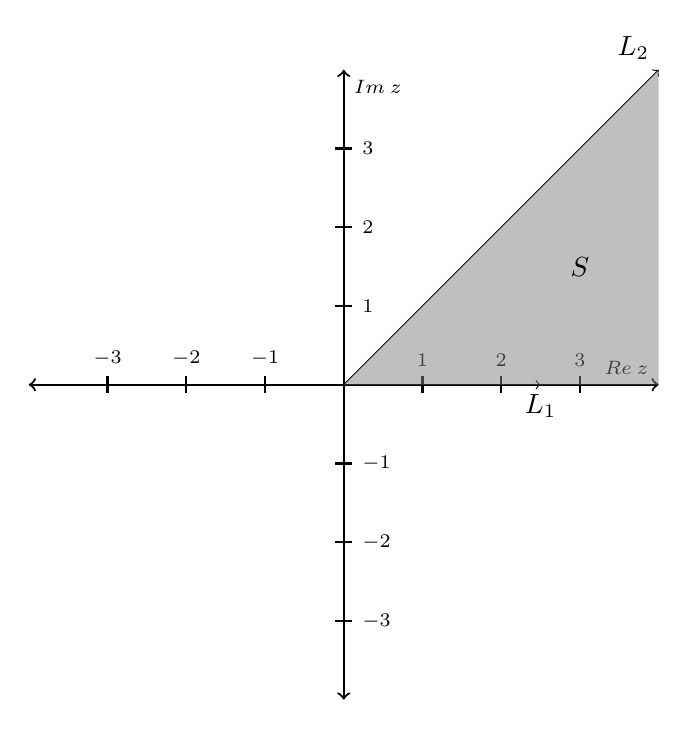
\begin{tikzpicture}
    \begin{scope}[thick,font=\scriptsize]
    \draw [<->] (-4,0) -- (4,0) node [above left]  {$Re\:z$};
    \draw [<->] (0,-4) -- (0,4) node [below right] {$Im\:z$};
    \foreach \n in {-3,...,-1,1,2,...,3}{
        \draw (\n,-3pt) -- (\n,3pt)   node [above] {$\n$};
        \draw (-3pt,\n) -- (3pt,\n)   node [right] {$\n$};
    }
    \end{scope}
    \draw [->] (0,0) -- (4, 4) node [above left] {$L_2$};
    \draw [->] (0,0) -- (2.5, 0) node [below] {$L_1$};
    \path [fill=gray,semitransparent] (0,0) -- (4, 4) -- (4, 0);
    \node [black] at (+3,+1.5) {$S$};
    \end{tikzpicture}
    \\Clearly the boundary of $S$ is given by $\{z\in\mathbb{C}: arg\:z\in\{0,\frac{\pi}{4}\}\}\subseteq S$.
    \\Therefore $S$ contains all its boundary points and hence is not open. So $S$ is not a domain.
\end{center}

\newpage
{\Large\textbf{f.}} Let $S =\{z\in\mathbb{C}: |z - 4|\geq |z|\} =\{z\in\mathbb{C}: |z - 4|\geq |z - 0|\}$.
\begin{center}
    \doublespacing
    Then $S$ consists of all the points whose distance from 4 is at least their distance from 0.
    \\To put it in terms easier to visualize:
    \\$z\in S$ if and only if the following holds. 
    \\$\sqrt{(z - 4)(\overline{z - 4})}\geq \sqrt{z\overline{z}}$. So $(z - 4)(\overline{z} - 4)\geq z\overline{z}$.
    \\Therefore $z\overline{z} - 4z - 4\overline{z} + 16\geq z\overline{z}$ and $16\geq 4(z +\overline{z})$.
    \\Finally we get $4\geq 2 Re\:z$ and $Re\:z\leq 2$.
    \break
    \\So $S =\{z\in\mathbb{C}: Re\:z\leq 2\}$.
    \\This makes sense geometrically as if $Re\:z > 2$ then $z$ will be closer to 4 than to 0. This is due to both 0 and 4 being on the real line making $Im\:z$ irrelevant as it will have the same effect on the distance from both 0 and 4.
    \\So $S$ consists of all the points on and to the left of the line $L: Re\:z = 2$
    \break
    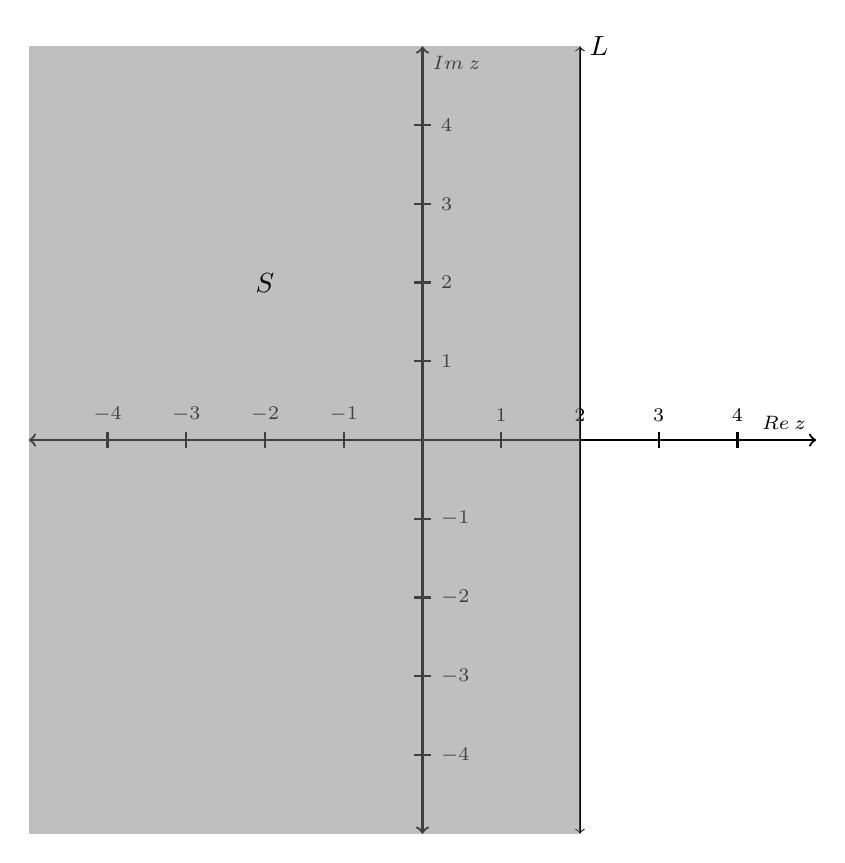
\begin{tikzpicture}
    \begin{scope}[thick,font=\scriptsize]
    \draw [<->] (-5,0) -- (5,0) node [above left]  {$Re\:z$};
    \draw [<->] (0,-5) -- (0,5) node [below right] {$Im\:z$};
    \foreach \n in {-4,...,-1,1,2,...,4}{
        \draw (\n,-3pt) -- (\n,3pt)   node [above] {$\n$};
        \draw (-3pt,\n) -- (3pt,\n)   node [right] {$\n$};
    }
    \end{scope}
    \draw [<->] (2,-5) -- (2, 5) node [right] {$L$};
    \path [fill=gray,semitransparent] (2, -5) -- (2, 5) -- (-5, 5) -- (-5, -5);
    \node [black] at (-2,+2) {$S$};
    \end{tikzpicture}
    \\Clearly the boundary of $S$ is given by $\{z\in\mathbb{C}: Re\:z = 2\}\subseteq S$.
    \\Therefore $S$ contains all its boundary points and hence is not open. So $S$ is not a domain.
\end{center}


\newpage
\section*{12.6}
\begin{center}
    \doublespacing
    Let $S\subseteq\mathbb{C}$ be an arbitrary set of complex numbers.
    \\We know that $z$ is a boundary point of $S$ if $z$ is not an interior or exterior point of $S$.
    \\In order for $z$ to be an interior point of $S$ there must exist some $\epsilon > 0$ such that $V_{\epsilon} (z)\subseteq S$.
    \\In order for $z$ to be an exterior point of $S$ there must exist some $\epsilon > 0$ such that $V_{\epsilon} (z)\subseteq S^c$.
    \\Therefore if $z$ is not a boundary point of $S$ then there must exist some $\epsilon > 0$ where either $V_{\epsilon} (z)\subseteq S$ or $V_{\epsilon} (z)\subseteq S^c$.
    \begin{itemize}
        \item Assume that $S$ is open:
    \end{itemize}
    Then $S$ does not contain any of its boundary points.
    \\Consider some arbitrary point $z\in S$. We know $z$ can not be a boundary point of $S$.
    \\So there exists an $\epsilon > 0$ where we have either $V_{\epsilon} (z)\subseteq S$ or $V_{\epsilon} (z)\subseteq S^c$.
    \\Take any $\epsilon > 0$ then we know $z\in V_{\epsilon} (z)$, so $V_{\epsilon} (z)\not\subseteq S^c$ since $z\in S$.
    \\So there does not exist an $\epsilon > 0$ where $V_{\epsilon} (z)\subseteq S^c$.
    \\Therefore we must have that there exists an $\epsilon > 0$ where $V_{\epsilon} (z)\subseteq S$.
    \\This means that $z$ is an interior point of $S$.
    \\This was true for arbitrary $z\in S$ and is therefore true for all $z\in S$.
    \\So every point in $S$ is an interior point.
    \begin{itemize}
        \item Assume that every point in $S$ is an interior point:
    \end{itemize}
    Then if $z\in S$ we have that $z$ can not be a boundary point because $z$ is already an interior point.
    \\Consider some arbitrary boundary point $w$ of $S$. Then it must be $w\notin S$.
    \\Otherwise $w$ would be an interior point of $S$ and hence not a boundary point of $S$.
    \\This was true for an arbitrary boundary point $w$ of $S$ and is therefore true for every boundary point of $S$.
    \\Therefore $S$ does not contain any of its boundary points.
    \\So $S$ is open.
    \break
    \\So we have that $S$ is open if and only if every point in $S$ is an interior point of $S$ \qedsymbol
\end{center}


\newpage
\section*{14.2}

\begin{center}
    \doublespacing
    Recall that for a complex number $z = x + iy$ we know $\overline{z} =\overline{x + iy} = x - iy$, also recall that $i^2 = -1$.
    \\Further recall the binomial theorem where for $z_1, z_2\in\mathbb{C}$ we know \[(z_1 + z_2)^n =\sum _{k=0}^n\binom{n}{k} z_1^k z_2^{n-k}\]
\end{center}

{\Large\textbf{a.}} Let $f(z) = z^3 + z + 1$.
\begin{center}
    \doublespacing
    Then if $z = x + iy$ we have: \[f(z) = f(x + iy) = (x + iy)^3 + (x + iy) + 1 =\Bigg{(}\sum _{k=0}^3\binom{3}{k} x^k (iy)^{3-k}\Bigg{)} + (x + iy) + 1 =\]
    \[(x^3 + 3ix^2 y - 3x y^2 - iy^3) + (x + iy) + 1 = (x^3 - 3x y^2 + x + 1) + i(3x^2 y - y^3 + y)\]
    So $f(z) = f(x + iy) = u(x, y) + iv(x, y)$ where:
    \[u(x, y) = x^3 - 3x y^2 + x + 1\]
    and
    \[v(x, y) = 3x^2 y - y^3 + y\]
\end{center}

{\Large\textbf{b.}} Let $f(z) =\frac{\overline{z}^2}{z} =\frac{\overline{z}^2\overline{z}}{z\overline{z}} =\frac{\overline{z}^3}{z\overline{z}}$.
\begin{center}
    \doublespacing
    Then if $z = x + iy$ we have: \[f(z) = f(x + iy) =\frac{(\overline{x + iy})^3}{(x + iy)(\overline{x + iy)}} =\frac{(x - iy)^3}{(x + iy)(x - iy)} =\frac{1}{x^2 - ixy + ixy - i^2 y} (x - iy)^3 =\]
    \[\frac{1}{x^2 + y^2}\Bigg{(}\sum _{k=0}^3\binom{3}{k} x^k (-iy)^{3-k}\Bigg{)} =\frac{1}{x^2 + y^2} (x^3 - 3i x^2 y - 3 x y^2 + iy^3) =\frac{x^3 - 3x y^2}{x^2 + y^2} + i\frac{y^3 - 3x^2 y}{x^2 + y^2}\]
    So $f(z) = f(x + iy) = u(x, y) + iv(x, y)$ where:
    \[u(x, y) =\frac{x^3 - 3x y^2}{x^2 + y^2}\]
    and
    \[v(x, y) =\frac{y^3 - 3x^2 y}{x^2 + y^2}\]
\end{center}


\newpage
\section*{14.3}
\begin{center}
    \doublespacing
    Recall that for a complex number $z = x + iy$ we know $x = Re\:z =\frac{z +\overline{z}}{2}$ and $y = Im\:z =\frac{z -\overline{z}}{2i}$.
    \break
    \\Now let $f(z) = f(x + iy) = (x^2 - y^2 - 2y) + i(2x - 2xy)$.
    \\We can substitute with the equations given before to get:
    \[f(z) = \Big{(}(\frac{z +\overline{z}}{2})^2 - (\frac{z -\overline{z}}{2i})^2 - 2\frac{z -\overline{z}}{2i}\Big{)} + i\Big{(}2\frac{z +\overline{z}}{2} - 2 (\frac{z +\overline{z}}{2})(\frac{z -\overline{z}}{2i})\Big{)} =\]
    \[\Big{(}\frac{(z +\overline{z})^2}{2^2} -\frac{(z -\overline{z})^2}{(2i)^2} -\frac{i(z -\overline{z})}{i^2}\Big{)} + i\Big{(}z +\overline{z} - 2 \frac{i(z +\overline{z})(z -\overline{z})}{4i^2}\Big{)} =\]
    \[\frac{z^2 + 2z\overline{z} +\overline{z}^2}{4} +\frac{z^2 - 2z\overline{z} +\overline{z}^2}{4} + i(z -\overline{z}) + iz + i\overline{z} + \frac{i^2(z +\overline{z})(z -\overline{z})}{2} =\]
    \[\frac{z^2 +\overline{z}^2}{2} + 2iz -\frac{z^2 - z\overline{z} + z\overline{z} -\overline{z}^2}{2} =\frac{z^2 +\overline{z}^2}{2} + 2iz - \frac{z^2 -\overline{z}^2}{2} =\]
    $\overline{z}^2 + 2iz$ \qedsymbol
\end{center}


\newpage
\section*{14.6}
\begin{center}
    \doublespacing
    Let $f(z) = z^2$. Then for $z = x + iy$ we have $f(x + iy) = (x + iy)^2 = x^2 + 2ixy + (iy)^2 = (x^2 - y^2) + i(2xy)$.
    \\So $f(z) = f(x + iy) = u(x, y) + i v(x, y)$ where $u(x, y) = x^2 - y^2$ and $v(x, y) = 2xy$.
    \\Therefore if $z\in\mathbb{C}$ where $z = x + iy$ such that $x^2 - y^2 = c_1$ for some $c_1 < 0$ then $u(x,y) = Re\:f(z) = c_1$.
    \\Furthermore if $z\in\mathbb{C}$ where $z = x + iy$ such that $2xy = c_2$ for some $c_2 < 0$ then $v(x,y) = Im\:f(z) = c_2$.
    \\Let us first look at the case where $z = x + iy$ and $x^2 - y^2 = c_1$:
    \\Notice that if $y > 0$ then as $x$ increases we have $v = 2xy$ increases.
    \\Also notice that if $y < 0$ then as $x$ decreases we have $v = 2xy$ increases.
    \break
    \begin{tikzpicture}
    \begin{scope}[thick,font=\scriptsize]
    \draw [<->] (-4,0) -- (4,0) node [above left]  {$x$};
    \draw [<->] (0,-4) -- (0,4) node [below right] {$y$};
    \end{scope}
    \pgfmathsetmacro{\a}{-1}
    \draw plot[domain=-2:2] ({\a*sinh(\x)},{\a*cosh(\x)});
    \draw plot[domain=-2:2] ({\a*sinh(\x)},{-\a*cosh(\x)});
    \path [fill=black] (0, 1) circle (0.06);
    \path [fill=black] (0, -1) circle (0.06);
    \draw [thick,->] (-2, 2.23) -- (-1.999, 2.2289) {};
    \draw [thick,->] (2, 2.23) -- (2.001, 2.2309) {};
    \draw [thick,->] (-1.999, -2.2289) -- (-2, -2.23) {};
    \draw [thick,->] (2.001, -2.2309) -- (2, -2.23) {};
    \node [below left] at (0, 1) {$-c_1$};
    \node [above left] at (0, -1) {$c_1$};
    \end{tikzpicture}
    \begin{tikzpicture}
    \begin{scope}[thick,font=\scriptsize]
    \draw [<->] (-4,0) -- (4,0) node [above left]  {$u$};
    \draw [<->] (0,-4) -- (0,4) node [below right] {$v$};
    \end{scope}
    \draw [-] (-2, -4) -- (-2, 4) {};
    \draw [thick,->] (-2, -2.001) -- (-2, -2) {};
    \draw [thick,->] (-2, 1.999) -- (-2, 2) {};
    \path [fill=black] (-2, 0) circle (0.06);
    \node [below right, black] at (-2, 0) {$c_1$};
    \end{tikzpicture}
    \\Now let us look at the case where $z = x + iy$ and $2xy = c_2$:
    \\Notice that as $|x|$ increases it must be that $|y|$ decreases in order for $2xy = c_2$ to stay constant.
    \\This means that when $|x|$ increases (causing $x^2$ to increase and $y^2$ to decrease) we have $u = x^2 - y^2$ increases.
    \break
    \begin{tikzpicture}
    \begin{scope}[thick,font=\scriptsize]
    \draw [<->] (-4,0) -- (4,0) node [above left]  {$x$};
    \draw [<->] (0,-4) -- (0,4) node [below right] {$y$};
    \end{scope}
    \pgfmathsetmacro{\c}{-0.5}
    \draw plot[domain=-2:2] ({\c*(sinh(\x) + cosh(\x))},{\c*(sinh(\x) - cosh(\x))});
    \draw plot[domain=-2:2] ({-\c*(sinh(\x) + cosh(\x))},{\c*(cosh(\x) - sinh(\x))});
    \draw [thick,->] (-2.499, 0.103) -- (-2.5, 0.1029) {};
    \draw [thick,->] (-0.499, 0.501) -- (-0.5, 0.5) {};
    \draw [thick,->] (2.499, -0.103) -- (2.5, -0.1029) {};
    \draw [thick,->] (0.499, -0.501) -- (0.5, -0.5) {};
    \end{tikzpicture}
    \begin{tikzpicture}
    \begin{scope}[thick,font=\scriptsize]
    \draw [<->] (-4,0) -- (4,0) node [above left]  {$u$};
    \draw [<->] (0,-4) -- (0,4) node [below right] {$v$};
    \end{scope}
    \draw [-] (-4, -2) -- (4, -2) {};
    \draw [thick,->] (-2.001, -2) -- (-2, -2) {};
    \draw [thick,->] (1.999, -2) -- (2, -2) {};
    \path [fill=black] (0, -2) circle (0.06);
    \node [below right, black] at (0, -2) {$c_2$};
    \end{tikzpicture}
\end{center}

\end{document}
